\documentclass{article}
\usepackage[utf8]{inputenc}
\usepackage{indentfirst}
\usepackage{titling}
\usepackage{geometry}
\usepackage{graphicx}
\graphicspath{ {./Images/} }
\usepackage[shortlabels]{enumitem}
\usepackage{fancyhdr}
\usepackage{ulem}
\usepackage[dvipsnames]{xcolor}
\usepackage{amssymb}
\usepackage{listings}
\usepackage{color}

\definecolor{dkgreen}{rgb}{0,0.6,0}
\definecolor{gray}{rgb}{0.5,0.5,0.5}
\definecolor{mauve}{rgb}{0.58,0,0.82}

\lstset{frame=tb,
  language=Java,
  aboveskip=3mm,
  belowskip=3mm,
  showstringspaces=false,
  columns=flexible,
  basicstyle={\small\ttfamily},
  numbers=none,
  numberstyle=\tiny\color{gray},
  keywordstyle=\color{blue},
  commentstyle=\color{dkgreen},
  stringstyle=\color{mauve},
  breaklines=true,
  breakatwhitespace=true,
  tabsize=3
}

\def\ojoin{\setbox0=\hbox{$\bowtie$}%
  \rule[-.02ex]{.25em}{.4pt}\llap{\rule[\ht0]{.25em}{.4pt}}}
\def\leftouterjoin{\mathbin{\ojoin\mkern-5.8mu\bowtie}}
\def\rightouterjoin{\mathbin{\bowtie\mkern-5.8mu\ojoin}}
\def\fullouterjoin{\mathbin{\ojoin\mkern-5.8mu\bowtie\mkern-5.8mu\ojoin}}

\renewcommand\maketitlehooka{\null\mbox{}\vfill} %para centralizar verticalmente
\renewcommand\maketitlehookd{\vfill\null}
\pagestyle{fancy}
\fancyhf{}
\rfoot{\thepage}
\lfoot{ 
\includegraphics[scale=0.01]{UA.jpg} José Mendes 107188 LEI}
\geometry{
  a4paper,
  headheight=4cm,
  top=5.5cm,
  bottom=4.5cm,
  footskip=4cm
}


\title{Inteligência Artificial}
\author{José Mendes 107188}
\date{2023/2024}

\begin{document}


\begin{titlepage}
    \maketitle
    \begin{center}
        
\includegraphics[scale=0.4]{UA.png}
    \end{center}
    \thispagestyle{empty} %remove o count da pagina
\end{titlepage}

\pagebreak

\section{Noções de Programação Declarativa}

\subsection{Programação Declarativa}

A Programação Declarativa abstrai-se da implementação, focando-se
apenas na descrição do que se pretende fazer, enquanto faz uso de dois
paradigmas:
\begin{itemize}
  \item \textbf{Programação Funcional}, baseado em funções/calculo-lambda, a entidade central é a função;
  \item \textbf{Programação em Lógica}, baseado em lógica de primeira ordem, a entidade central é o predicado;
\end{itemize}


\subsection{Paradigma Imperativo}

O fluxo de operações é especialmente sequenciado de operações com
foco na forma como as tarefas são executadas (\textbf{instrução}). Podemos \textbf{alterar
o conteúdo em memória} e ainda (instruções de afetação/atribuição) e ainda
\textbf{realizar análise de casos} (if-then-else, switch/case, \dots), \textbf{processamento
iterativo} (while, repeat, for, \dots) e ter associados \textbf{sub-programas} (procedimentos,
funções).

\begin{flushleft}
\textbf{Exemplo:} SQL é uma linguagem declarativa, uma vez que nos seus comandos apenas descrevemos o que queremos obter.
Assim, o programador é abstraído da forma como as operações são executadas na prática, ficando essa tarefa a cargo
do compilador.
\end{flushleft}

\subsection{Paradigma Declarativo}

\begin{center}
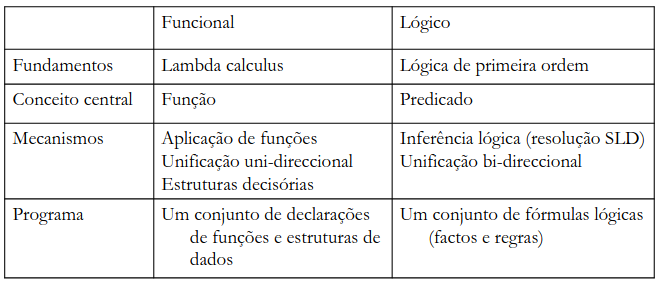
\includegraphics[scale=0.5]{1}
\end{center}

A sua origem data da segunda metade do século XX, mas ainda hoje é amplamente usada e
até está em crescimento em áreas como a Inteligência Artifical.

\pagebreak

\subsection{Programação Funcional}

Possibilidade de definir funções localmente e sem nome. Por exemplo as
funções lambda presentes em Lisp e Python.

\subsection{Programação em Lógica}

Um programa é uma teoria sobre um domínio. Por exemplo, temos
\textbf{socrates é um homem}, $homem(socrates)$ e, um \textbf{homem é mortal}, $homem(X) :- \hspace{1mm} mortal(X)$.
Se perguntarmos se \textbf{socrates é mortal}, $mortal(socrates)$, a resposta é \uline{sim}.

\subsection{Atitude do programador}

A programação declarativa, dada a sua elevada expressividade, é pouco
compatível com aproximações empíricas (ou seja, tentativa e erro) à programação.
Primeiro é preciso pensar bem na estrutura do problema antes de começar a teclar.

\vspace{2mm}

\begin{flushleft}
  \textbf{Passos a seguir:} Perceber o problema $\rightarrow$ Desenhar o programa $\rightarrow$
  Escrevê-lo $\rightarrow$ Rever e testar
\end{flushleft}

\subsection{Características da Programação Funcional}

\begin{itemize}
  \item A entidade central é a função;
  \item A noção de função é diretamete herdada da matemática (ao contrário das
  linguagens imperativas, que pode ser muito diferente);
  \item A estrutura de controlo fundamental é a "aplicação de funções";
  \item A noção de "tipo da função" captura a noção matemática de
  domínio (de entrada e saída);
  \item Os elementos do domínio de entrada e saída podem ser funções;
\end{itemize}

\subsection{Função}

Tem valores de entrada (domínio) e valores de saída (contradomínio).

\begin{center}
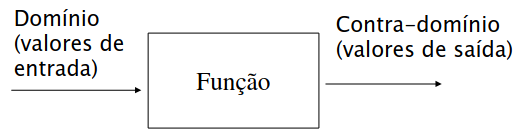
\includegraphics[scale=0.4]{2}
\end{center}

\subsection{Programação em Lógica}

Um programa numa linguagem baseada em lógica representa uma teoria sobre um
problems. Um programa é uma sequência de frases ou fórmulas representando
\textbf{factos} (informação sobre objetos do problema/domínio de aplicação) e \textbf{regras}
(leis gerais sobre esse problema/domínio). Implicitamente as frases estão reunidas
nume grande conjunção, e cada frase está universalmente quantificada. Portanto,
\textbf{programação declarativa}.

\pagebreak

\section{Programação ao estilo funcional em Python}

\subsection{Python}

Criada no final dos anos 90, é uma linguagem de programação interpretada,
iterativa, portável, funcional, orientada a objetos e de implementação aberta.
Tem como principais objetivos: simplicidade sem prejuizo da utilidade,
programação modular, legibilidade, desenvolvimento rápido, facilidade de integração,
nomeadamente com outras linguagens. Apresenta-se como uma linguagem \textbf{multi-paradigma}:
\begin{itemize}
  \item \textbf{Programação funcional:} Expressões lambda, funções de ordem superior,
  listas com sintaxe simples, iteradores, \dots
  \item \textbf{Programação OO:} Classes, objetos, métodos, herança, \dots
  \item \textbf{Programação imperativa/modular:} Atribuição, sequências,
  condicionais, ciclos, \dots
\end{itemize}

\subsubsection{Python vs Java}

Comparativamente ao JAVA revela-se menos consisa porque os espaços são sintaticamente
relevantes e o código, não compilado para código nativo (interpretado), demora mais tempo a
executar (diferença residual), no entanto apresenta uma maior facilidade de desenvolvimento e
legibilidade.

\subsubsection{Áreas de aplicação}

As principais áreas de aplicação são: interligação de sistemas, aplicações gráficas,
aplicações para bases de dados, multimédia, internet protocol/web e
robótica e inteligência artificial.

\subsection{Dados, ou "objetos"}

\begin{flushleft}
  \textbf{Objeto:} no contexto de Pyhton, esta designação é
  aplicada a qualquer dado que possa ser armazenado
  numa variável, ou passado como parâmetro a uma
  função.
\end{flushleft}

Cada objeto é caracterizado por uma identidade/referência (identifica a posição
de memória onde está armazenado), um tipo e um valor. Alguns tipos de
objetos podem ter atributos e métodos, outros (classes) podem ter
sub-tipos (sub-classes).

\begin{center}
  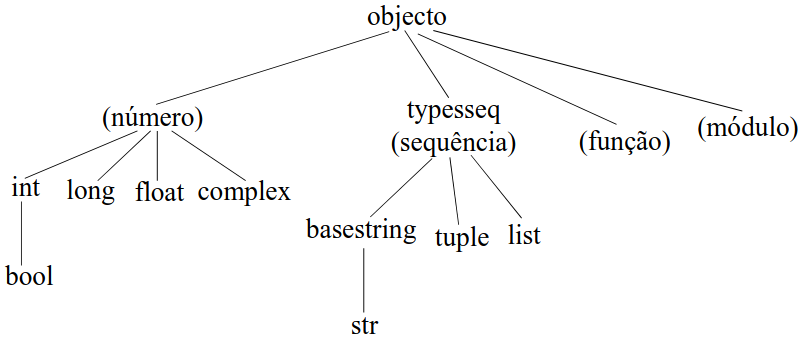
\includegraphics[scale=0.3]{3}
\end{center}

Alguns destes são imutáveis, como as \textbf{str} e \textbf{tuple}. Para determinar o tipo de um objeto utiliza-se a função pré-definida \textbf{type()}.

\pagebreak

\subsection{Variáveis}

As variáveis guardam objetos, mas não são declaradas (inicializadas apenas) nem têm tipos
associados (o tipo é do objeto!). Praticamente tudo pode ser atribuido a uma variável, incluindo
funções, módulos e classes. Similar as linguagens imperativas, e ao contrário das
funcionais, o valor de uma variável pode ser alterado. Não se pode ler o valor de uma variável
se este não tiver sido previamente inicializado.

\subsection{Intrução de atribuição}

Tal como é habitual na programação imperativa, e ao
contrário do habitual na programação declarativa,
Python possui instrução de atribuição.

\begin{flushleft}
  \textbf{Exemplo:}
  \begin{lstlisting}
    n = 10
    a = b = c = 0
    x = 7.25
    cad = "cadeia"
    t = (n, x)
    l = [1, 2, 'quatro', 5.0]
  \end{lstlisting}
\end{flushleft}

Pode user a operação de atribuição para decompor estruturas:
\begin{lstlisting}
  triplo = (1, 2, 3)
  (i, j, k) = triplo
\end{lstlisting}

\subsection{Operadores}

Operadores comuns matemáticos e lógicos. É importante saber que objetos de
tipos diferentes nunca são iguais (exceto os diferentes tipos de números).

\subsubsection{Operadores lógicos}

Na conjunção e disjunção, o segundo elemento só é avaliado de for necessário para determinar
o resultado.

\begin{lstlisting}
  if False and a: # a nao e avaliado
    ...

  if True or a: # a nao e avaliado
    ...
\end{lstlisting}

\pagebreak

\subsection{Acesso a sequências}

Os elementos das sequências são acedidos
através de índices inteiros consecutivos (primeiro elemento tem índice 0).

\vspace{2mm}

É possível extrair “fatias” das sequências. A indexação é circular, pelo que podemos aceder a
índices negativos.

\begin{lstlisting}
  # [inf:sup] retorna a sequencia entre os indices inf e sup-1 (uma opia da lista)

  # Para fazer uma copia integral da lista usa-se [:]
\end{lstlisting}

\begin{flushleft}
  \textbf{Detalhe importante:}  instrução de atribuição, em vez de copiar valores, limita-se
  a associar um dado identificador a um dado objecto. Desta forma, a atribuição
  da variável x a uma variável y, apenas tem como resultado associar y
  ao mesmo objecto que x já estava associada. No caso dos objetos
  mútaveis, temos de ter cuidado:

  \begin{lstlisting}
    a = [1, 2, 3]
    b = a
    b[1:2] = []
    print(a) # [1, 3]
  \end{lstlisting}
\end{flushleft}

\subsection{Definição de funções}

Funções sem return, retornam None, são também conhecidas como procedimentos. As funções podem
ser recursivas e são objetos do tipo \textbf{function}.

\vspace{2mm}

Os parâmetros são passados às funções segundo um mecânismo "passagem por valor"
("call by value"). \uline{Os parâmetros são passados por referêcia, não cópias!}. 

\vspace{2mm}

Se atribuirmos um novo objeto a uma variável passada por
parâmetro, essa atribuição ocorre apenas no espaço de nomes da função (imagem à
esquerda). Se modificarmos um objeto passado por parâmetro (por
exemplo, apagar um elemento de uma lista), isto não altera a
referência do objeto, e portanto vai permanecer após o
retorno da função (imagem à direita).

\begin{center}
  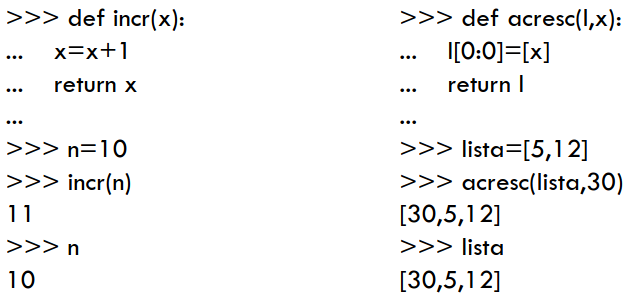
\includegraphics[scale=0.3]{4}
\end{center}

O problema anterior resolve-se trabalhando sobre uma cópia local,
no caso de uma lista l, podemos usar l[:], que dá uma cópia integral.

\pagebreak

Podemos passar parâmetros com valores por defeito, podendo se, na chamada,
omitir alguns parâmetros.

\begin{lstlisting}
  def abc(arg1, arg2=True, arg3=None):
    ...
  # Quando so queremos passar um dos args por defeito devemos indicar o seu nome
  abc(1, arg3=3)
\end{lstlisting}

\subsection{Funções Recursivas}

\end{document}